%!TEX root = ./template-skripsi.tex

\subsection{Sprint 1 Report}
	
	Pada sprint pertama ini story yang di pilih untuk di uraikan pada sprint kali ini adalah pencatatan pemberian pakan. Rentang waktu sprint ini sedikit lebih lama dari sprint lainnya sekitar 2-3 minggu, yang mana sprint lainnya hanya 1-2 minggu. Perbedaan tersebut terjadi karena penulis melakukan training terhadap bahasa dan framework yang akan digunakan dalam pengembangan sistem, sekaligus memberi waktu penulis untuk melakukan pendaftaran dan penulisan pada penelitian.
	
	Tujuan dari sprint-1 adalah membuat CRUD berbentuk API untuk sebuah fitur pencatatan pemberian pakan. Dimulai dari mendesain database, desain struktur sistem, desain class pada sistem, membuat program dari desain yang sudah ada, dan yang terakhir adalah melakukan deployment sistem ke server. Penggunaan platform Github Projects untuk mempermudah manajemen task dan progress seperti pada \textbf{Gambar \ref{fig:github_projects_sprint01}}.
	
\begin{figure}[H]
	\centering
	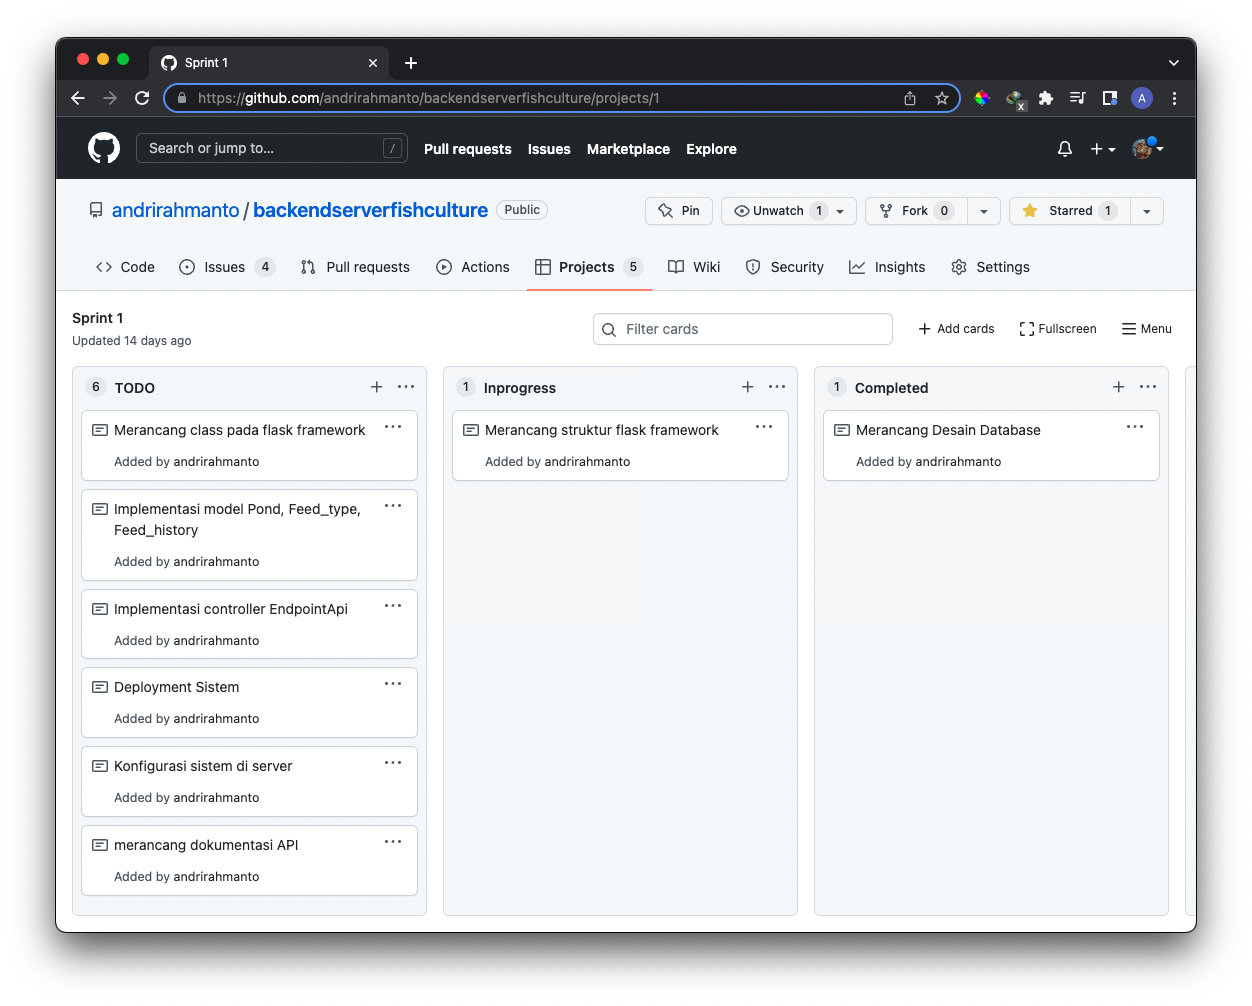
\includegraphics[width=1\textwidth]{gambar/Sprint01/github_project_sprint01.png}
	\caption{Github Projects Sprint-1}
	\label{fig:github_projects_sprint01}
\end{figure}

	Dari \textbf{Gambar \ref{fig:github_projects_sprint01}} diatas, terdapat 4 kolom yang menggambarkan fase dari task tersebut. 4 fase itu adalah to do, in progress, completed, dan tested. To do menandakan fase dimana task baru hanya didaftarkan pada list. In progress menandakan fase dimana task sedang dalam proses pengerjaan oleh developer. Completed merupakan fase dimana task sudah selesai dikerjakan. Dan tested merupakan fase dimana task tertentu telah di test oleh developer dan scrum master.
	
\begin{enumerate}[a).]

	\item{Merancang Database}
	
		Desain Database atau biasa disebut Entity Relationship Diagram (ERD) pada sprint-1 menggambarkan struktur data dan relasi antar data yang akan disimpan pada database. 
	
		\begin{figure}[H]
			\centering
			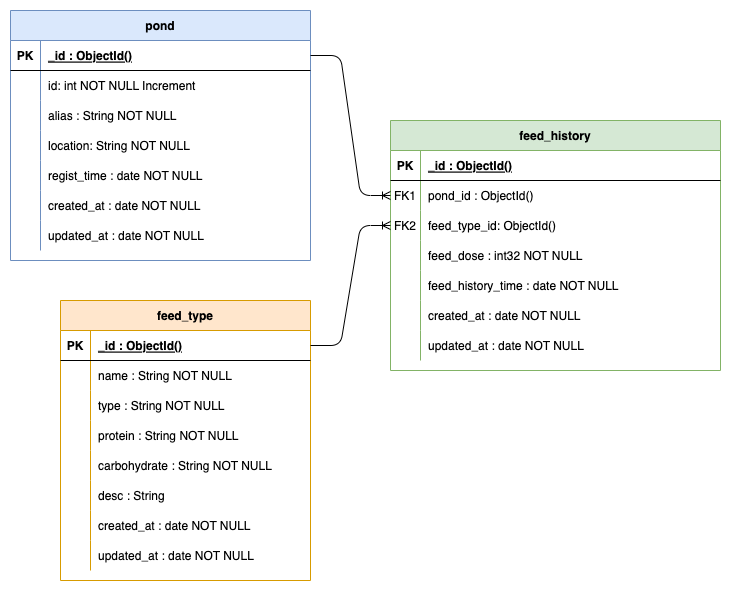
\includegraphics[width=0.7\textwidth]{gambar/Sprint01/diagram database/database.png}
			\caption{ERD Database Sprint-1}
			\label{fig:erd_database_sprint01}
		\end{figure}
		
		Terdapat 3 tabel yang dibutuhkan untuk menunjang fitur pemberian pakan. Tabel pond tabel pond berfungsi untuk menyimpan data terkait kolam, dimana ada beberapa field yaitu nama dan lokasi kolam. Tabel \textit{feed\_type} berfungsi menyimpan data terkait tipe pakan, dimana field yang disimpan adalah nama pakan, tipe pakan, kandungan protein pakan dalam bentuk persentase, kandungan karbohidrat pakan dalam bentuk persentase, dan keterangan tambahan. Tabel \textit{feed\_history} berfungsi untuk menyimpan data terkait pemberian pakan, dimana field yang disimpan adalah id kolam, id tipe pakan, dosis pakan, dan waktu pemberian pakan.
		
	\item{Merancang Struktur Flask Framework}
	
	Rancangan struktur flask framework menggambarkan direktori-direktori pada sistem yang akan di buat. terdapat 4 direktori penting yaitu database, resource, static, template. Direktori database berisi file yang berkaitan dengan database mongodb yaitu, koneksi database dan model data pada database. Direktori resource deskripsi routes dan controller untuk setiap logic API endpoint. Direktori static berisi hal-hal yang dibutuhkan untuk styling sebuah halaman html, yang biasanya berisi css file dan javascript file. Direktori template merupakan tempat penulis menyimpan html file. Pembagian direktori tersebut bertujuan untuk mempermudah pengolahan dalam pengembangan sistem kedepannya.
	
\begin{forest}
  pic dir tree,
  where level=0{}{% folder icons by default; override using file for file icons
    directory,
  },
  [fishapi
    [\_\_init\_\_.py, file]
    [database
    	[\_\_init\_\_.py, file]
	[db.py,file]
	[models.py,file]
    ]
    [index.wsgi, file]
    [resources
      [\_\_init\_\_.py, file]
      [controller
      	  [\_\_init\_\_.py, file]
	  [feed\_history.py,file]
	  [feed\_type.py,file]
	  [pond.py,file]
      ]
      [routes.py,file]
    ]
    [settings.cfg, file]
    [static]
    [templates]
  ]
\end{forest}
		
	\item{Merancang Class Diagram}
	
	Class Diagram menggambarkan kelas-kelas yang akan dipakai oleh sistem. Umumnya terdapat 3 kelas pada setiap module yaitu class model, controller, dan view. Untuk sprint-1 setiap modul hanya terdapat 2 class yaitu model, dan controller.
	
	\begin{figure}[H]
		\centering
		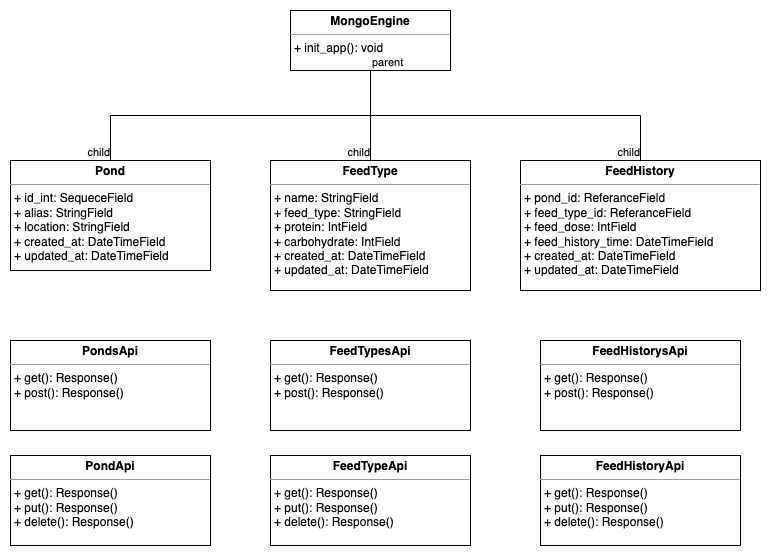
\includegraphics[width=0.9\textwidth]{gambar/Sprint01/class diagram/class_diagram.png}
		\caption{Class Diagram Sprint-1}
		\label{fig:class_diagram_sprint01}
	\end{figure}
	
	Pada \textbf{Gambar \ref{fig:class_diagram_sprint01}} setiap module terdapat 3 class. Semisal module Pond terdapat 1 class untuk model dan 2 class controller API. class model merupakan class yang mewarisi sifat MongoEngine.Document yang merupakan sebuah package pada python untuk mempermudah manipulasi database. Sedangkan class controller API merupakan class yang dibuat untuk mendeskripsikan logic yang akan dijalankan setiap client mengakses API Endpoint.
	
	\item{Implementasi model Pond, Feed\_type, Feed\_history}
	
	Implementasi model dilakukan menggunakan bantuan package Mongoengine yang mana mengharuskan menjadikan Mongoengine.Document sebagai parent dari class tersebut. Pada setiap atribut class harus didefinisikan terhadap jenis field yang telah disediakan oleh Mongoengine.
	
	\begin{enumerate}[1).]
		\item{Model Pond}
			\begin{lstlisting}
class Pond(db.Document):
    id_int = db.SequenceField(required=True)
    alias = db.StringField(required=True)
    location = db.StringField(required=True)
    created_at = db.DateTimeField(default=datetime.datetime.now)
    updated_at = db.DateTimeField(default=datetime.datetime.now)
			\end{lstlisting}
		\item{Model Feed\_type}
			\begin{lstlisting}
class FeedType(db.Document):
    name = db.StringField(required=True)
    feed_type = db.StringField(required=True)
    protein = db.IntField(required=True)
    carbohydrate = db.IntField(required=True)
    desc = db.StringField()
    created_at = db.DateTimeField(default=datetime.datetime.now)
    updated_at = db.DateTimeField(default=datetime.datetime.now)
			\end{lstlisting}
		\item{Model Feed\_history}
			\begin{lstlisting}
class FeedHistory(db.Document):
    pond_id = db.ReferenceField(Pond, required=True)
    feed_type_id = db.ReferenceField(FeedType, required=True)
    feed_dose = db.IntField(required=True)
    feed_history_time = db.DateTimeField(default=datetime.datetime.now)
    created_at = db.DateTimeField(default=datetime.datetime.now)
    updated_at = db.DateTimeField(default=datetime.datetime.now)
    			\end{lstlisting}
	\end{enumerate}
	
	\item{Implementasi Controller EndpointAPI}
	
	\begin{enumerate}[1).]
		\item{Add Routes}
			\begin{lstlisting}
def initialize_routes(api):
    # pond
    api.add_resource(PondsApi, '/api/ponds')
    api.add_resource(PondApi, '/api/ponds/<id>')
			\end{lstlisting}
		\item{PondsApi}
			Class PondsApi
			\begin{lstlisting}
class PondsApi(Resource):
    def get(self):
        objects = Pond.objects()
        response = []
        for pond in objects:
            pond = pond.to_mongo()
            response.append(pond)
        response_dump = json.dumps(response, default=str)
        return Response(response_dump, mimetype="application/json", status=200)

    def post(self):
        body = {
            "alias": request.form.get("alias", None),
            "location": request.form.get("location", None),
        }
        pond = Pond(**body).save()
        id = pond.id
        return {'id': str(id)}, 200
    			\end{lstlisting}
		\item{PondApi}
			\begin{lstlisting}
class PondApi(Resource):
    def put(self, id):
        body = {
            "alias": request.form.get("alias", None),
            "location": request.form.get("location", None),
            "updated_at": datetime.datetime.utcnow()
        }
        Pond.objects.get(id=id).update(**body)
        return '', 200

    def delete(self, id):
        pond = Pond.objects.get(id=id).delete()
        return '', 200

    def get(self, id):
        objects = Pond.objects.get(id=id)
        pond = objects.to_mongo()
        response_dump = json.dumps(pond, default=str)
        return Response(response_dump, mimetype="application/json", status=200)
    			\end{lstlisting}
	\end{enumerate}
	
	\item{Deployment Sistem}
	
	Sistem pada akhirnya dijalankan pada server agar dapat diakses client melalui akses internet. Pertama yang dilakukan adalah mengunggah repositori sistem ke repositori github. Repositori github terdapat pada \textit{\textbf{https://github.com/andrirahmanto/backendserverfishculture/tree/sprint\_01}}. Lalu setelahnya adalah menghubungkan personal computer penulis ke server dengan metode SSH (Secure Shell Connection). Menghubungkan dengan metode ssh dilakukan melalui terminal pada dengan cara
\begin{lstlisting}
ssh <user>@<ip_address_server>
\end{lstlisting}
dan masukan password ketika diminta.

	Selanjutnya hubungkan server dengan repositori github yang sudah dibuat menggunakan metode git remote. 
\begin{lstlisting}
mkdir /var/www/html/<name_your_repo>
git init
git remote add origin <link_github>
git pull origin main
\end{lstlisting}
dengan begitu server telah memiliki repo yang sama dengan yang ada di personal komputer. Langkah selanjutnya diikuti dengan penginstalan package yang dipakai pada sistem.

	\item{Konfigurasi Sistem pada Server}

	Konfigurasi bertujuan untuk menjalankan sistem yang sudah di upload ke server. Tahapan pertama konfigurasi adalah memastikan bahwa sistem berbentuk package agar dapat di import. kemudian buat file index.wsgi seperti dibawah ini
\begin{lstlisting}
import logging
import sys

logging.basicConfig(stream=sys.stderr)
sys.path.insert(0, '/var/www/html/fishapi')

from fishapi import create_app
application = create_app()
\end{lstlisting}
	index.wsgi nantinya akan didaftarkan ke file httpd.conf pada server agar sistem dapat dieksekusi oleh server.
\begin{lstlisting}
WSGIDaemonProcess /fishapi python-path=/opt/rh/rh-python38/root/lib/pyt$
WSGIProcessGroup /fishapi
WSGIApplicationGroup %{GLOBAL}
WSGIScriptAlias /fishapi /var/www/html/fishapi/index.wsgi
WSGIScriptReloading on
<Directory "/var/www/html/fishapi/fishapi">
	AllowOverride All
	Options +ExecCGI
	AddHandler cgi-script .cgi .pl .py
	Order allow,deny
	allow from all
</Directory>

Alias /fishapi/static /var/www/html/fishapi/fishapi/static
<Directory /var/www/html/fishapi/fishapi/static>
	AllowOverride All
	Order allow,deny
	allow from all
</Directory>
\end{lstlisting}
Setelahnya lakukan restart pada apache pada server dengan menjalankan:
\begin{lstlisting}
systemctl restart http
\end{lstlisting}
Setelah konfigurasi selesai, sistem akan di test pada browser dengan melakukan request.
\begin{figure}[H]
		\centering
		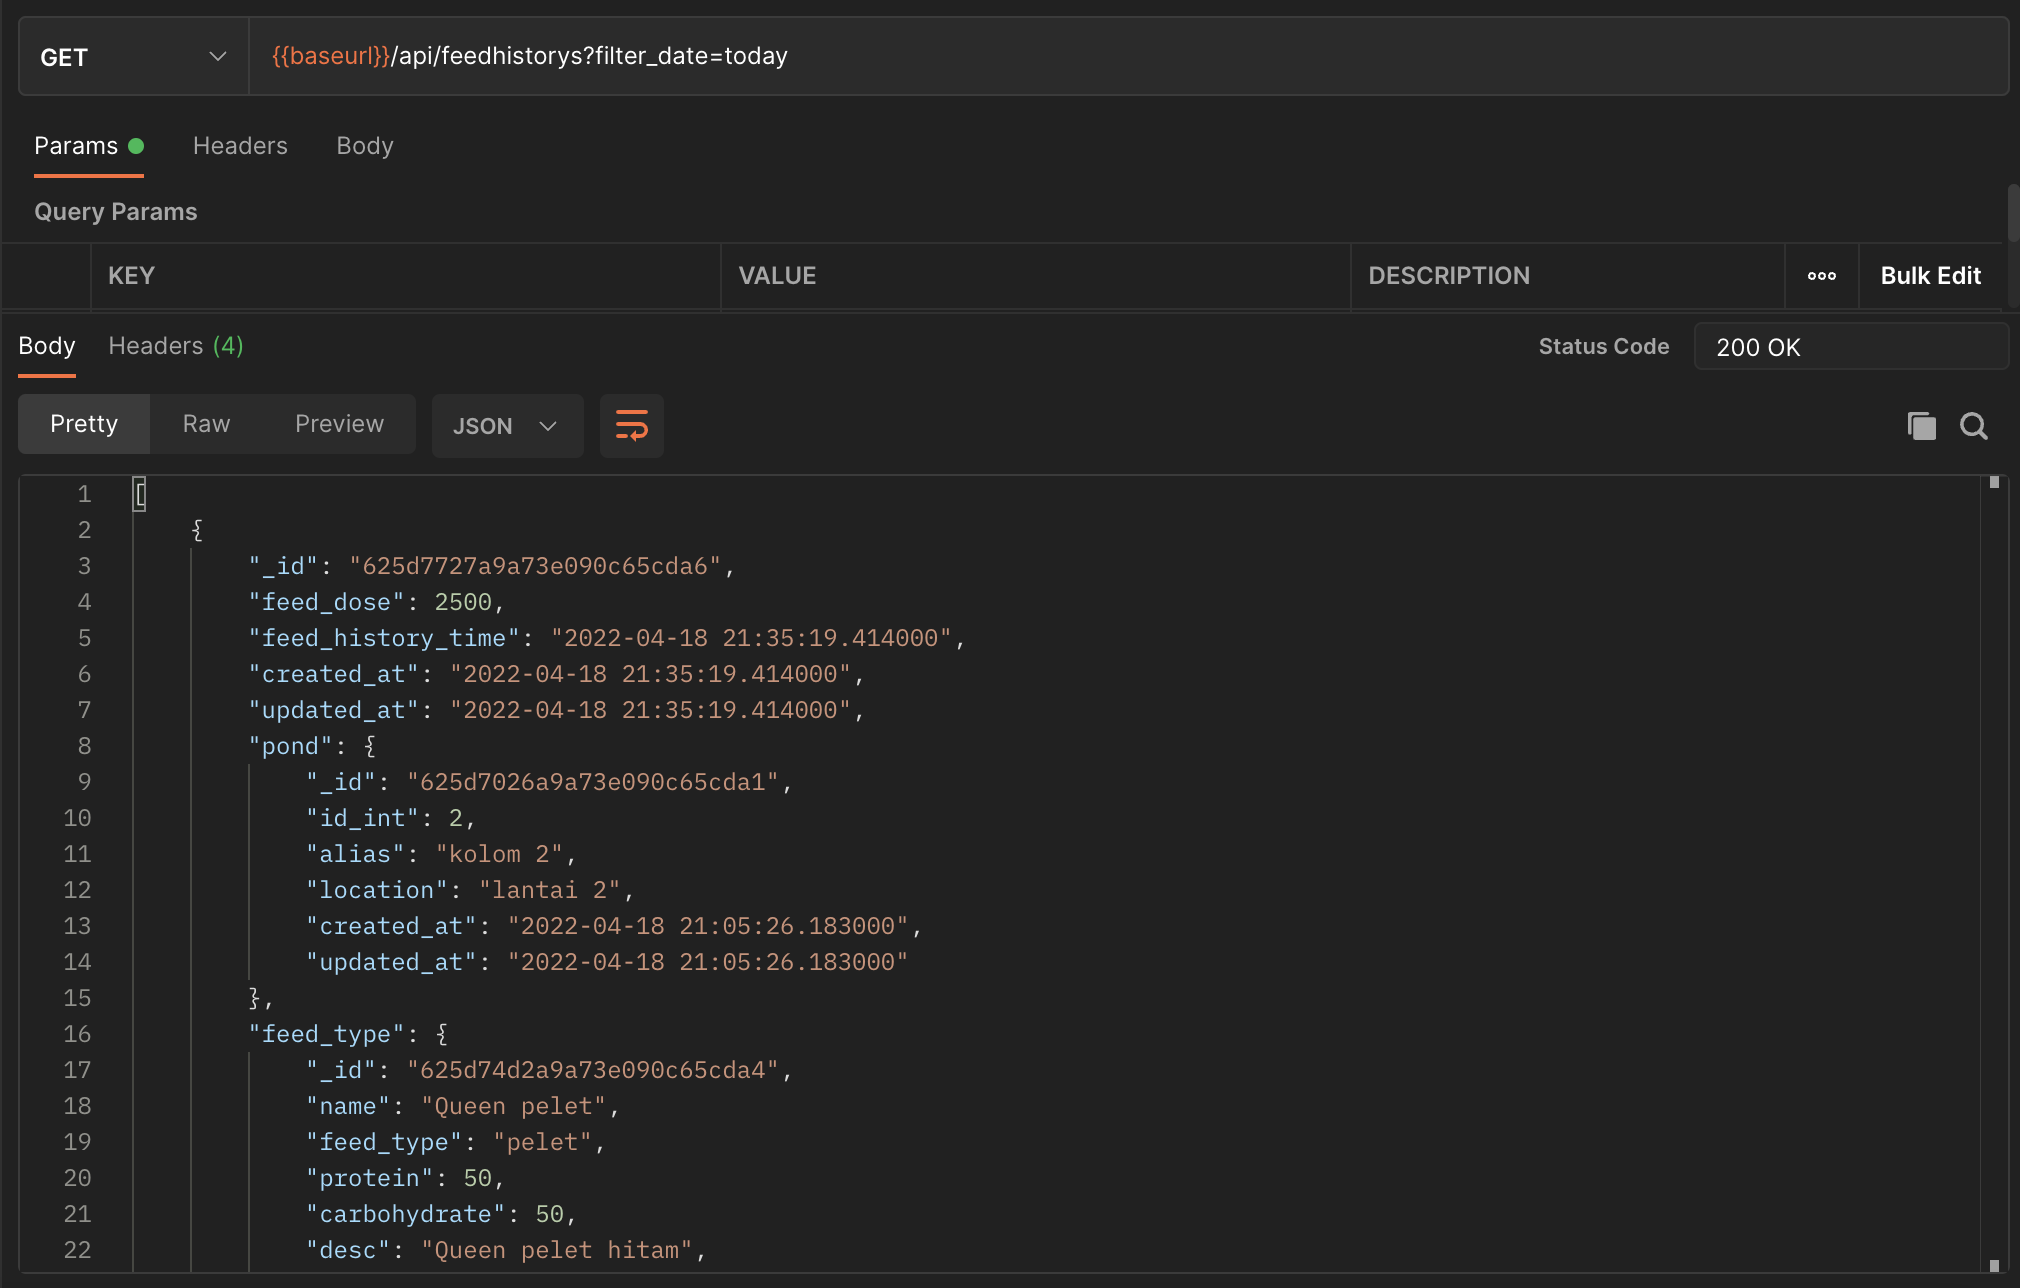
\includegraphics[width=0.9\textwidth]{gambar/Sprint01/request_get.png}
    		\caption{\textit{Request Get \emph{pemberian pakan} Postman}}
		\label{fig:request_get}
\end{figure}
	
	
	\item{Dokumentasi API}
	
	Dokumentasi API dibuat menggunakan postman, yang mana dapat diakses melalui link \textit{\textbf{https://documenter.getpostman.com/view/11714934/UVysybzY}}.
	berikut beberapa contoh request dan response yang diberikan server:
	request cURL:
\begin{lstlisting}
curl --location --request GET 'http://jft.web.id/fishapi/api/ponds'
\end{lstlisting}
	response json:
\begin{lstlisting}
[
  {
    "_id": "625d7026a9a73e090c65cda1",
    "id_int": 2,
    "alias": "alpha",
    "location": "blok 1",
    "shape": "bundar",
    "material": "beton",
    "length": 0,
    "width": 0,
    "diameter": 1.4,
    "height": 1,
    "build_at": "2022-04-18 21:05:26.183000",
    "image_name": "kolam_1655141767.jpeg",
    "area": 1.5399999999999998,
    "image_link": "http://127.0.0.1:5000/api/ponds/image/625d7026a9a73e090c65cda1",
    "volume": 1.5399999999999998
  },
  { "_id": "625d7033a9a73e090c65cda2",.....},
  { "_id": "62a62163e445ffb9c5f746f3",......},
  { "_id": "62a955888911334402ddb3b3",.....},
  {"_id": "62a9a466299f257e382a8295",.....}
]
\end{lstlisting}	

	\item{Unit Testing}
	
	Unit Testing dilakukan pada akhir sprint. Adapun hasil dari unit testing yang telah dilaksanakan dapat dilihat pada tabel di bawah ini:
	
\begin{table}[H]
	\centering
	\caption{Unit Testing Sprint 1}
	\label{table:unittesting_sprint1}
	\begin{tabular}{|l|l|ll|l|}
\hline
\multirow{2}{*}{No} & \multirow{2}{*}{Skenario Pengujian} & \multicolumn{2}{l|}{Kesesuaian}     & \multirow{2}{*}{Kesimpulan} \\ \cline{3-4}
                    &                                     & \multicolumn{1}{l|}{Sesuai} & Tidak &                             \\ \hline
1  & Pencatatan pemberian pakan          & \multicolumn{1}{l|}{\CheckmarkBold}&& Diterima \\\hline
2  & Merubah data pemberian pakan          & \multicolumn{1}{l|}{\CheckmarkBold}&& Diterima \\\hline
3  & Mendapatkan list data pemberian pakan          & \multicolumn{1}{l|}{\CheckmarkBold}&& Diterima \\\hline
4  & Mendapatkan detail data pemberian pakan          & \multicolumn{1}{l|}{\CheckmarkBold}&& Diterima \\\hline
5  & Menghapus data pemberian pakan          & \multicolumn{1}{l|}{\CheckmarkBold}&& Diterima \\\hline
\end{tabular}
\end{table}
\end{enumerate}